
\documentclass{report}

\usepackage{graphicx}  % For including images
\usepackage{amsmath}   % For mathematical symbols and environments
\usepackage{hyperref}  % For hyperlinks
\usepackage{wrapfig}  % For wrapping text around figures

% Command to create the title page
\newcommand{\report}[3]{
    \title{#1}
    \author{#2}
    \date{#3}
    \maketitle
}

\begin{document}

% Create the title page
\report{Solar sail Mercury}{Roberto Lucchesi 1744941}{\today}


\newpage

\section*{Introduction}
The aim of this project is to design a solar sail mission to Mercury. The spacecraft is equipped with a solar sail, which is a large, lightweight mirror that reflects sunlight to propel the spacecraft. The sail is controlled by adjusting the angle of the sail relative to the Sun. The spacecraft is launched from Earth and is required to reach a stable orbit around Mercury. 
In particular, the optimal control that minimizes the time of flight is sought. 

\subsection*{Dynamical model}
The dynamical framework employed is the one of the patched conics for interplanetary travel. 
A 2D planar polar coordinate system is used, with the Sun at the origin and the spacecraft moving in the plane of the ecliptic.
In this framework, the spacecraft dynamic can be written as:
\begin{equation*}
    \begin{bmatrix}
        \dot{r} \\
        \dot{\theta} \\
        \dot{v_r} \\
        \dot{v_{\theta}}
    \end{bmatrix}
    =
    \begin{bmatrix}
        v_r \\
        v_{\theta}/r \\
        v_{\theta}^2/r - \mu/r^2 + F_r \\
        -v_r v_{\theta}/r + F_{\theta}
    \end{bmatrix}
\end{equation*}
where $F_r$ and $F_{\theta}$ are the radial and tangential components of the solar radiation pressure force that can be
written with respect to the sail angle $\boldsymbol{\alpha}$ as:
\begin{equation*}
    \begin{bmatrix}
        F_r \\
        F_{\theta}
    \end{bmatrix}
    =
    \begin{bmatrix}
        \beta/r^2 \cos^3(\alpha) \\
        \beta/r^2 \sin(\alpha) \cos^2(\alpha)
    \end{bmatrix}
\end{equation*}
and $\beta$ defined as:
\begin{equation*}
    \beta = \frac{2 W_E}{c\; \sigma}
\end{equation*}
with $W_E$ the solar radiation pressure at Earth, $c$ the speed of light, and $\sigma = 20 \; g/m^2$ the sail loading factor.

\section*{Optimal control problem}
The optimal control problem is formulated through the calculus of variations and the Mayer-Lagrange formulation.
In this context, the functional to minimize is:
\begin{equation*}
    J = t_f
\end{equation*}
while the Hamiltonian is found as:
\begin{equation*}
    H = \lambda_r v_r + \lambda_{\theta} v_{\theta}/r + \lambda_{v_r} (v_{\theta}/r) + \lambda_{v_{\theta}} (v_{\theta}^2/r - \mu/r^2 + F_r) + \lambda_{v_{\theta}} (-v_r v_{\theta}/r + F_{\theta}) + \lambda_k(-1)
\end{equation*}
where $\boldsymbol{\lambda}$ are the costate variables.
Their time derivative are found differentiating the Hamiltonian with respect to the state variables:
\begin{equation*}
    \begin{bmatrix}
        \dot{\lambda_r} \\
        \dot{\lambda_{\theta}} \\
        \dot{\lambda_{v_r}} \\
        \dot{\lambda_{v_{\theta}}} \\
        \dot{\lambda_k}
    \end{bmatrix}
    =
    -\frac{\partial H}{\partial \boldsymbol{x}}
\end{equation*}
In particular, we can observe:
\begin{equation*}
    \begin{bmatrix}
        \dot{\lambda_{\theta}} \\
        \dot{\lambda_{k}} \\ 
    \end{bmatrix}
    = 
    \begin{bmatrix}
            0 \\
            0 \\
    \end{bmatrix}
\end{equation*}
so that this two costate variables are constant along the trajectory.
%%%%%%%%%%%%%%%%%%%%%%%%%%%%%%%%%%%%%%%%%%%%%%%%%%%%%%%%%%%%%%%%%%%%%%%%%%%%%%%%%%%%%%%%%%%%%%%%%%%%%%%%%%%%%%%%%%%%%%%%%%%%%%%
\subsection*{Optimal control angle}
The control angle $\boldsymbol{\alpha}$ is the optimal control to be found. The optimal value is computed by seeking for a stationary point in the Hamiltonian:

\begin{equation*}
\frac{dH}{d\alpha }= -3\frac{\lambda_{vr} \beta}{r^2}\cos^2(\alpha)\sin(\alpha) + \frac{\lambda_{v_{\theta}}\beta}{r^2}(-2\sin^2(\alpha)\cos(\alpha) + \cos^2(\alpha))  = 0 
\end{equation*}
That has for solution, in terms of the costate variables:
\begin{equation*}
    \begin{cases}
        \alpha = \pm \;\pi/2 \rightarrow \textrm{T} = 0\\
        \alpha = \arctan(\frac{-3\lambda_{vr} \pm \sqrt{9\lambda_{vr}^2 + 8\lambda_{v_{\theta}}}}{4\lambda_{v_{\theta}}}) 
    \end{cases}
\end{equation*}


%%%%%%%%%%%%%%%%%%%%%%%%%%%%%%%%%%%%%%%%%%%%%%%%%%%%%%%%%%%%%%%%%%%%%%%%%%%%%%%%%%%%%%%%%%%%%%%%%%%%%%%%%%%%%%%%%%%%%%%%%%%%%%%
\subsection*{Initial conditions and constraints}
The spacecraft is assumed to be along Earth trajectory at initial time, and shall be at Mercury orbit at the final time, 
 so:
\begin{equation*}
    \begin{bmatrix}
        r(0) \\
        \theta(0) \\
        v_r(0) \\
        v_{\theta}(0)
    \end{bmatrix}
    =
    \begin{bmatrix}
        R_E \\
        0 \\
        0 \\
        v_E
    \end{bmatrix}
    \quad \quad \quad
    \begin{bmatrix}
        r(t_f) \\

        v_r(t_f) \\
        v_{\theta}(t_f)
    \end{bmatrix}
    =
    \begin{bmatrix}
        R_M \\

        0 \\
        v_M
    \end{bmatrix}
\end{equation*}
The sail angle is constrained to be between $-\pi/2$ and $\pi/2$. The final state is regarded as the
costraint function $\phi$.\\
Other final constraints are imposed on the costate equations by:
\begin{equation*}
    \boldsymbol{\lambda_f} = \frac{dJ}{d\boldsymbol{x}_f} + \boldsymbol{\lambda}\frac{d\phi}{d\boldsymbol{x}_f}
    \rightarrow \; \lambda_k = 1,\;\; \lambda_{\theta} = 0
\end{equation*}
and on the Hamiltonian by:
\begin{equation*}
    H_f = -\frac{dJ}{dt_f} - \boldsymbol{\lambda}\frac{d\phi}{dt_f} \rightarrow H_f = - 1
\end{equation*}

\subsection*{Approach to the solution}
The initial conditions on the remaining uknown costates and the final time is sought. Letting:
\begin{equation*}
    \boldsymbol{S_0^*} = \begin{bmatrix}
        \lambda_r(0) \\
        \lambda_{v_r}(0) \\
        \lambda_{v_{\theta}}(0) \\
        t_f
    \end{bmatrix}
\end{equation*}
the initial condition that leads to the optimal solution, several methods can be employed to aid in the search by numerical methods.
\subsubsection{Transversality conditions}

By multiplying the functional J by a constant k > 0, the constraint on the Hamiltonian is relaxed and can be rewritten through an inequality constraint on the final time:
\begin{equation*}
    H_f < 0
\end{equation*}
\subsubsection{Adjoint scalability}
Letting $\boldsymbol{\lambda_0^*}$ be the optimal initial costate, it can be demonstrated that
$\boldsymbol{\lambda_k^*} = k \boldsymbol{\lambda_0^*}$ is also a valid solution. This property can be exploited to limit the search space for the 
costate solutions in the interval [-1, 1].

\subsubsection{Adimensionalitation}
Adimensionalizing the problem leads to a formulation less sensible to variations of order of magnitudes in the state variables. The following variables are defined:

\begin{equation*}
    \textrm{D} = 1 \; \textrm{AU} \quad \quad \quad \textrm{T such as} \; \; \frac{D^3}{T^2} = \mu 
\end{equation*}
Each relevant quantity is then divided by the corresponding dimensional quantity, so that the problem is rewritten in terms of adimensional variables.\\\\\\
Nevertheless, indirect methods are very sensitive to the initial guess, leading to failure in convergence or in constraint violation.\\\\ To solve this problem a \textbf {Particle Swarm Optimizator} as been 
employed to find a good initial guess for \textbf{fmincon}. Due to the costrained nature of the problem, the PSO algorithm has been modified to include the constraints in the optimization process as a penalty cost function. 
\subsection*{Results}
The solutions found by the PSO and fmincon algorithms are here plotted
% Table with dr, dvt and final time of the PSO solution
\begin{equation} 
    \boldsymbol{S^{PSO}_0 = \begin{bmatrix}
        -0.819788 \\
        -0.079609 \\
        -0.873044 \\
        9.249678 
    \end{bmatrix}}
\end{equation}
\begin{table}[h]
    \centering
    \begin{tabular}{|c|c|c|c|}
        \hline
        $dr(km)$ & $dv_\theta$(km/s) & $t_f(days)$  \\
        \hline
        1244085 & 0.100256 & 537.74 \\
        \hline
    \end{tabular}
    \caption{Final state difference between PSO and fmincon solutions}
\end{table}
\begin{figure}[h]
    \centering
    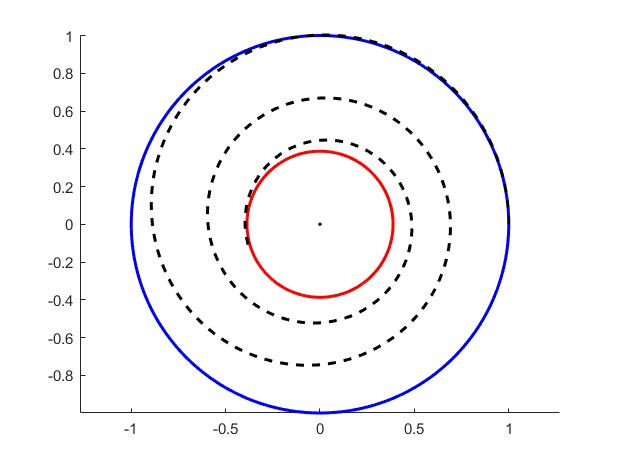
\includegraphics[width=0.49\textwidth]{results/pso_opt.jpg}
    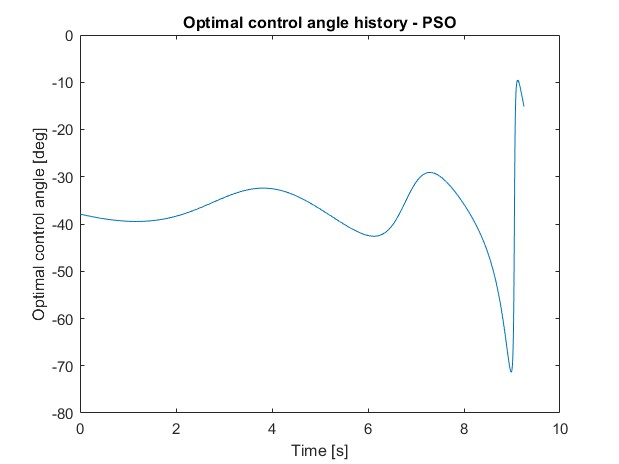
\includegraphics[width=0.49\textwidth]{results/a_pso.jpg}
    \caption{Optimal trajectory and control angle found by PSO}
\end{figure}\\
The PSO algorithm has been able to find a good initial guess for the fmincon algorithm,  but the constraint violation is still not negligible.
\\
Using $S^{PSO}_0$ as initial guess for fmincon, the final state difference between is:
\begin{equation} 
    \boldsymbol{S^{fmin}_0 = \begin{bmatrix}
        -0.820850 \\
        -0.073196 \\
        -0.872466 \\
        9.348250 
    \end{bmatrix}}
\end{equation}
\begin{table}[h]
    \centering
    \begin{tabular}{|c|c|c|c|}
        \hline
        $dr(km)$ & $dv_\theta$(km/s) & $t_f(days)$  \\
        \hline
        34 & 0.000046 & 543.47 \\
        \hline
    \end{tabular}
    \caption{Final state difference between PSO and fmincon solutions}
\end{table}
\begin{figure}[h]
    \centering
    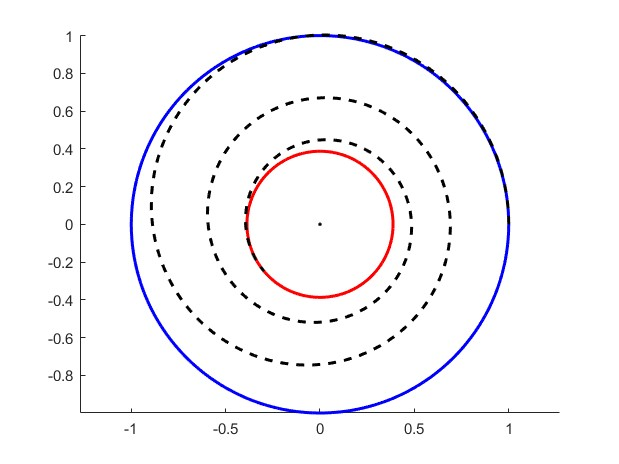
\includegraphics[width=0.49\textwidth]{results/fmincon_opt.jpg}
    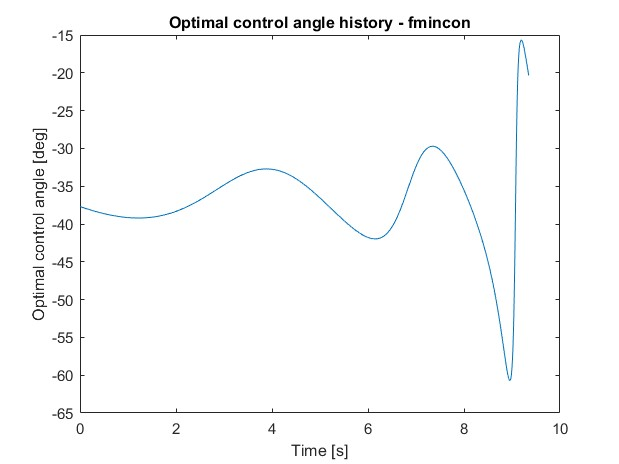
\includegraphics[width=0.49\textwidth]{results/a_fmin.jpg}
    \caption{Optimal trajectory and control angle found by PSO}
\end{figure}\\

\end{document}
